% -----------------------------------------------
% Template for ISMIR Papers
% 2016 version, based on previous ISMIR templates

% Requirements :
% * 6+1 page length maximum
% * 2MB maximum file size
% * Copyright note must appear in the bottom left corner of first page
% (see conference website for additional details)
% -----------------------------------------------

\documentclass{article}
\usepackage{ismir,amsmath,cite}
\usepackage{graphicx}
\usepackage{color}

% Title.
% ------
\title{Modulo7 : A full stack Music Information Retrieval And Structured Querying Engine}

% Note: Please do NOT use \thanks or a \footnote in any of the author markup

% Single address
% To use with only one author or several with the same address
% ---------------
%\oneauthor
% {Names should be omitted for double-blind reviewing}
% {Affiliations should be omitted for double-blind reviewing}

% Two addresses
% --------------
%\twoauthors
%  {First author} {School \\ Department}
%  {Second author} {Company \\ Address}

%% To make customize author list in Creative Common license, uncomment and customize the next line
%  \def\authorname{First Author, Second Author} 


% Three addresses
% --------------
\threeauthors
  {First Author} {Affiliation1 \\ {\tt author@ismir.edu}}
  {Second Author} {\bf Retain these fake authors in\\\bf submission to preserve the formatting}
  {Third Author} {Affiliation3 \\ {\tt author3@ismir.edu}}

%% To make customize author list in Creative Common license, uncomment and customize the next line
%  \def\authorname{First Author, Second Author, Third Author} 

% Four or more addresses
% OR alternative format for large number of co-authors
% ------------
%\multauthor
%{First author$^1$ \hspace{1cm} Second author$^1$ \hspace{1cm} Third author$^2$} { \bfseries{Fourth author$^3$ \hspace{1cm} Fifth author$^2$ \hspace{1cm} Sixth author$^1$}\\
%  $^1$ Department of Computer Science, University , Country\\
%$^2$ International Laboratories, City, Country\\
%$^3$  Company, Address\\
%{\tt\small CorrespondenceAuthor@ismir.edu, PossibleOtherAuthor@ismir.edu}
%}
%\def\authorname{First author, Second author, Third author, Fourth author, Fifth author, Sixth author}


\sloppy % please retain sloppy command for improved formatting

\begin{document}

%
\maketitle
%
\begin{abstract}
This paper describes a novel Music Information Retrieval and Structured Querying framework named Modulo7. Modulo7 is a full stack implementation (both client and server side software) which facilitates indexing variegated sources of music (midi, mp3, music xml and digitized sheet music files). Modulo7 implements a similarity search engine based on customized vector space representations of songs, an efficient indexing and persistent storage mechanism and an interface for querying attributes based on SQL(Structured Querying Language) like principles. The papers describes the implementation details and outlines speed up and scale up results over input sources and other MIR frameworks. \\\\
\textbf{Keywords : MIDI, Music XML, MP3, Music Retrieval, SQL}
\end{abstract}
%
\section{Introduction}\label{sec:introduction}

Given the explosive growth of Music Information Retrieval research, several approaches and software suits have been designed to tackle generic problems such as efficient indexing, similarity searches, archival methods, structured and un-structured querying,feature extraction, audio and digital signal processing. A vast majority of the MIR frameworks in academia tend to approach very specific problems and does not support scalability as a significant end goal in itself \cite{mirproblems}. Moreover, industry applications predominantly treat MIR applications based on collaborative filtering approaches \cite{amazonreco} and/or manual annotation \cite{musicgenomepandora} instead of structural analysis of music sources yet scales very well to large datasets. \\\\
Modulo7 is an attempt to capture the best features of both worlds. Modulo7 converts different music sources (midi, musicxml files, sheet music png/jpeg files and mp3) into a single unified symbolic representation. It indexes songs on global properties (artist, key signature, time signature etc) and provides a vector space implementation for similarity searches and querying based on the similie \cite{similie} platform and extended to include chords and polyphony. As a consequence, Modulo7 acts as an end to end software suite for Music Information Retrieval including client side querying, searching, indexing and persistent store mechanism.

%
\section{Relevant Work} \label{sec:relevantwork}

Music Information Retrieval is a vast and interdisciplinary body of work. In order to facilitate research in MIR, several software suits and frameworks have been developed in the academic community in the past. Notable amongst them are software suits like jMIR \cite{jMIR} for automatic feature extraction from audio and midi sources to be used as input into machine learning algorithms for genre classification, marsyas \cite{marsyas} and essentia \cite{essentia} for audio processing, humdrum \cite{humdrum} for automated musicological research, gamera \cite{gamera} for optical music recognition and symbol identification and SIMILIE \cite{similie} for melodic similarity analysis. \\\\
On top of the effort done by there has been significant effort undertaken by companies in the field of MIR with an emphasis on music recommendation. For instance Amazon implements a collaborative filtering approach by quantifying a consumer's shopping behavior \cite{amazonreco}. Pandora on the other hand utilizes an approach in which trained musicologists manually classify similarity between artists and songs \cite{pa}
\section{Software Aspects}\label{sec:architecture}

This section details the software aspects of the Modulo7 most notably its architecture and a typical work-flow description. 

\subsection{Software Architecture and Design}

The Modulo7 architecture can be visualized as \ref{fig:architecture} and is broadly divided into the following components. 

\begin{figure}
 {\framebox{
 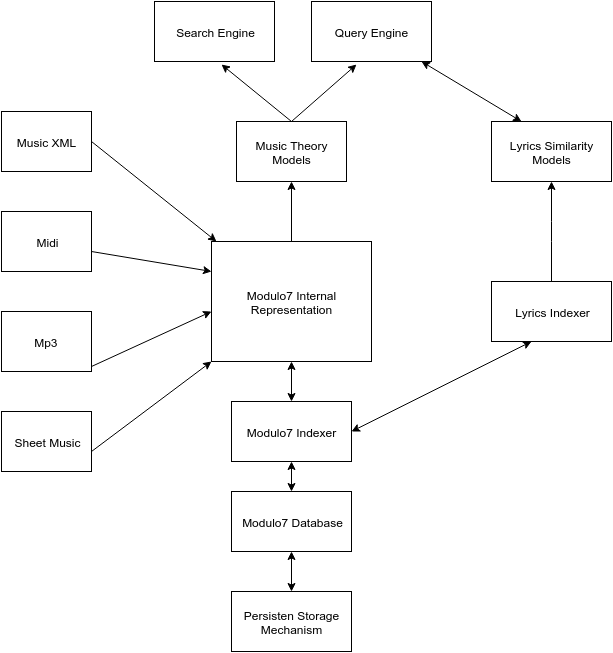
\includegraphics[width=\columnwidth]{Modulo7Architecture.png}}}
 \caption{A block diagram of the Modulo7 Architecture.}
 \label{fig:architecture}
\end{figure}

\begin{enumerate}
\item \textbf{Music Parsers: } Components that individually parse different music sources into a unified symbolic representation. as described in \ref{fig:document}. This object can be stored in memory or in a persistent serialized state via Apache Avro. Depending on the source of the file, the parser utilizes a different approach.
\begin{enumerate}
\item For mp3 files, the input is parsed into chromagrams using echonest API and then converted into symbolic format using the KKTonality profiles algorithm \cite{kkTonalityKeyFinding}. 
\item For Midi and MusicXML files, an in house parser is built. 
\item For Sheet Music, the Audiveris library is used to convert digitized sheet music to 

\end{enumerate}

\begin{figure}
 {\framebox{
 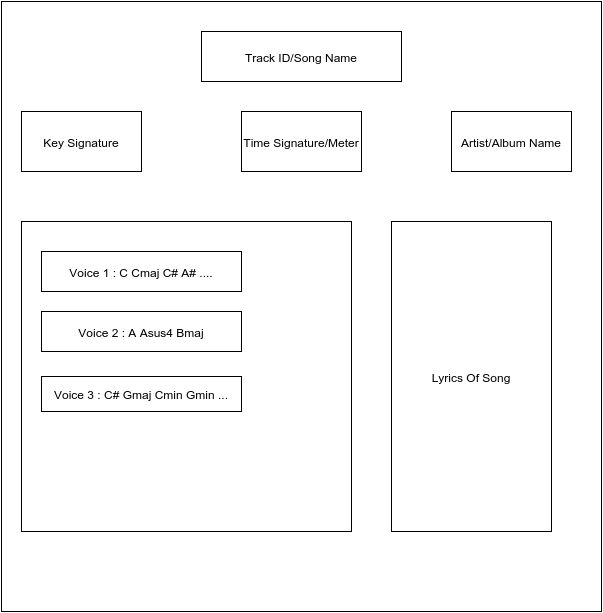
\includegraphics[width=\columnwidth, height=75mm]{DocumentStructureOfModulo7.png}}}
 \caption{Modulo7 internal representation.}
 \label{fig:document}
\end{figure}

\item \textbf{Music theory Models: } Modulo7 implements vector space models described in \cite{similie} with extensions to polyphonic music and chords using a template matching algorithm described in \cite{chord-detection}. This forms a mathematical formulation of music sources described in detail in section \ref{vecmodels} which is leveraged for querying and similarity searches.

\item \textbf{Client side Querying: } Modulo7 implements client side abstractions that exposes two modes of information retrieval. 
\begin{enumerate}
\item \textbf{Structured Querying: } The structured querying mode allows a user to make SQL like queries based on certain criteria or statistic that is quantified on music theoretic criteria. 
\item \textbf{Custom Search Engine: } Modulo7 exposes a search engine functionality but allowing for customized similarity metric choices as described in section \ref{searchengine} 
\end{enumerate}

\item \textbf{Lyrics Engine: } On top of providing support for music sources, Modulo7 also implements a standard text based retrieval model on lyrics of songs written in Apache Lucene.  

\end{enumerate}

\subsection{Workflow} 

The workflow can be defined as the steps of operations the user takes to initialize the Modulo7 system and expose the consumer to client facing querying options

\begin{enumerate}
\item Modulo7 is initialized by specifying a source directory. Every music source file inside the directory  is parsed and converted to either an in memory or persistent store version 
\end{enumerate}



\section{Vector Space Models for Music Sources} \label{vecmodels}


 
\section{Client Abstractions}

\subsection{Search Engine Functionality} \label{searchengine}

\section{Experimental Evaluation}

This section includes improvements that have been attained over existing frameworks and input sources. For the purposes of this experiment, existing datasets such as the Saarland dataset \cite{saarlandmsd}, the Wikifonia Dataset \cite{WikifoniaDataset} and the million song dataset \cite{msd}. 

\subsection{Indexing and Persistent Store Improvements}

\section{Conclusion and Future Work}


% For bibtex users:
\bibliography{ISMIRtemplate}

\end{document}
